\section{Sequence Planning via Parallel MCTS}\label{sec:sequence_planning}

We explore placement sequences using batched MCTS with parallel candidate evaluation to account for effects on subsequent placements.
Candidate placements are sampled, refined, and evaluated using the modules introduced in Sec.~\ref{sec:overview} (Fig.~\ref{fig:overview}).

\subsection{Batched Search Procedure}\label{sec:mcts}

\noindent \textbf{Batched Selection.}
We select evaluated, feasible children for batched expansion.
The colored paths in Fig.~\ref{fig:overview} terminate at the resulting expansion requests $b_j$.
For a child $\node$ reached by action $a$ from parent $\node_p$, we define the action prior over selectable child actions as
\begin{equation*}
 P(\node_p,a)=\operatorname{softmax}_{a}\!\left(w_\object\rho_\object^{\mathrm{pre}}(a)-w_E e(a)\right),
\end{equation*}
where $\rho_\object^{\mathrm{pre}}(a)$ is the fraction of object volume inside the target before simulation; $e(a)$ and the weights are defined in Sec.~\ref{sec:reward}.
This prior favors target containment and small equilibrium residuals.
Writing $N_{\node}=N(\node)$ and similarly for $Q,\hat N$, we adapt the Predictor Upper Confidence bounds applied to Trees (PUCT) rule used in AlphaGo Zero~\cite{silver2017mastering} for batched selection:
\begin{equation}
    \puct(\node)=\frac{N_{\node}Q_{\node}}{N_{\node}+\hat N_{\node}}
    +cP(\node_p,a)\frac{\sqrt{N_{\node_p}+\hat N_{\node_p}}}
         {1+N_{\node}+\hat N_{\node}},
    \label{eq:puct}
\end{equation}
where $c>0$ controls exploration toward less-visited alternatives, $\tmpvisit$ counts temporary reservations, and the first term is zero when its denominator is zero.
We use progressive widening~\cite{couetoux2011continuousuct} during tree search to expand the set of candidate placements as visits accumulate.
Temporary reservations $\hat N$ account for pending evaluations in selection scores during batch construction.
They are cleared after backpropagation and do not increase the completed-visit count used for progressive widening.

\noindent \textbf{Parallel Expansion and Evaluation.}
Requests (colored rows in Fig.~\ref{fig:overview}) are evaluated in parallel through $\initpose\to\poseopt\to\simul$.
Sampling chooses objects and initial poses; optimization refines the initial pose to improve target volume filling while minimizing static equilibrium residuals; simulation determines the settled successor state and reward.
MCTS compares the resulting placement sequences, coupling continuous refinement to future placement opportunities.

\noindent \textbf{Leaf Value Estimation and Backpropagation.}
For nonterminal, feasible leaves, we replace rollouts with $\hat V(\node)=\hat r\sum_{j=0}^{\depth_{\node}-1}\gamma^j$, where $\depth_{\node}$ counts future placements in the estimate, capped by remaining search depth and inventory.
The fixed hyperparameter $\hat r$ specifies a heuristic per-step reward for unexplored continuations and influences exploration through backpropagated returns.
Failed or terminal nodes have $\hat V=0$.
We propagate $r_{\node}+\gamma\hat V(\node)$, with incoming reward $r_{\node}$, toward the root, adding discounted ancestor rewards, updating $Q,N$, and clearing reservations.

\noindent \textbf{Action Selection and Replanning.}
Failed continuations can lower mean returns even when the search has found high-return feasible paths.
We therefore select the feasible root action maximizing
\begin{equation*}
  J(a)=(1-\beta)Q(\node_a)+\beta G(a),\qquad \beta\in[0,1].
\end{equation*}
Here $\node_a$ is the root child reached by $a$.
For each action $a$, we consider the deepest evaluated feasible paths from $\node_a$ within the search horizon and define
\begin{equation*}
 G(a)=\max_{(v_1,\ldots,v_m)}\sum_{t=1}^{m}\gamma^{t-1}r_{v_t},
\end{equation*}
where the maximum is over these paths, with $v_1=\node_a$.
Only observed rewards are included in $G(a)$, excluding $\hat V$. If no feasible continuation exists, $m=1$ and $G(a)=r_{\node_a}$.

We execute the selected placement, then replan with the observed successor state as the new root.

\begin{figure}[t]
  \centering
  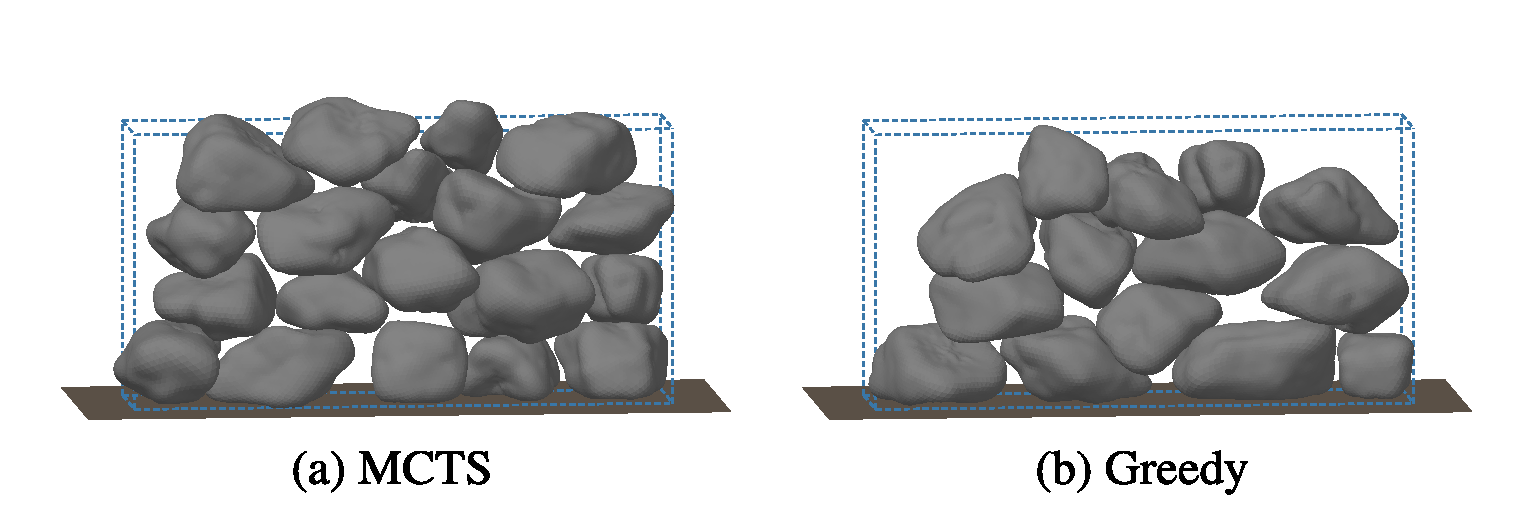
\includegraphics[width=0.95\columnwidth]{figures/mcts_example.eps}
  \caption{Wall construction using the same inventory of over 40 stones. MCTS places 19 stones ($44.0\%$ target volume filling); greedy stops at 14 ($36.1\%$), finding no further feasible placement. Blue dashed outlines show the target.}
  \label{fig:mcts_example}
\end{figure}


\subsection{Initial Pose Sampling}\label{sec:initial_pose_sampling}
The sampler $\initpose$ samples larger objects more often, uses finite orientation sets, and proposes initial placements near feasible target corners in empty scenes.
For object $i$, orientation $R$, and feasible planar location $\planar$, the score (Fig.~\ref{fig:score_map}) is
\begin{equation*}
  \score(\planar\mid i,R)
  =w_\text{s}\score_\text{s}+w_\text{f}\score_\text{f}
   +w_\text{b}\score_\text{b}-w_\text{h}\score_\text{h}-w_\text{d}\score_\text{d},
\end{equation*}
All weights are positive. The terms are: $\score_\mathrm{s}$, predicted bottom support fraction; $\score_\mathrm{f}$, unfilled area in the current construction layer beneath the footprint; $\score_\mathrm{b}$, proximity to the feasible placement boundary; $\score_\mathrm{h}$, mean height over predicted contact regions, min--max normalized across valid proposals for each object; and $\score_\mathrm{d}$, a bounded gap penalty between consecutive footprints (zero for the first placement).
The area and boundary terms favor filling empty regions and building inward~\cite{menezes2021rocks}.

We combine top-scoring proposals with sampling without replacement weighted by $\exp(\score/\tau)$, $\tau>0$.
The initial height keeps the lowest candidate point above the base plane and all objects with overlapping padded XY bounding boxes (Fig.~\ref{fig:score_map}(c)).
% Root proposals also use XY/yaw mutations. Displacement is measured from the
% initial pose, and height filtering uses the current construction level.
% Equilibrium rejection before simulation is defined in Reward Design.

\subsection{Simulation Module}\label{sec:simulation}
Dynamic validation tests settling and disturbance response beyond static force balance.
At every search depth, $\simul$ first simulates the candidate for a fixed time duration while holding existing objects fixed, then resets velocities and simulates the entire structure.
Settling requires a minimum time duration and sustained low kinetic energy; excessive accumulated motion or timeout causes rejection.

The settled scene defines $\state'=\transition(\state,\action)$.
From rest in $\state'$, independent disturbance trials apply a force of magnitude $\alpha m_{i_{k+1}}g$ at the center of mass of the candidate for $\Delta t_f$, in $n_d$ evenly spaced horizontal directions ($\alpha>0$, gravitational acceleration $g$).
With all objects dynamic, each trial must settle again without exceeding prescribed displacement limits relative to $\state'$; trials do not alter $\state'$.
GPU-accelerated subADMM~\cite{ji2025gpu} evaluates independent candidates in parallel.

% Delay the float to place Fig. 6 at the top of the right column.
\begin{figure}[t]
  \centering
  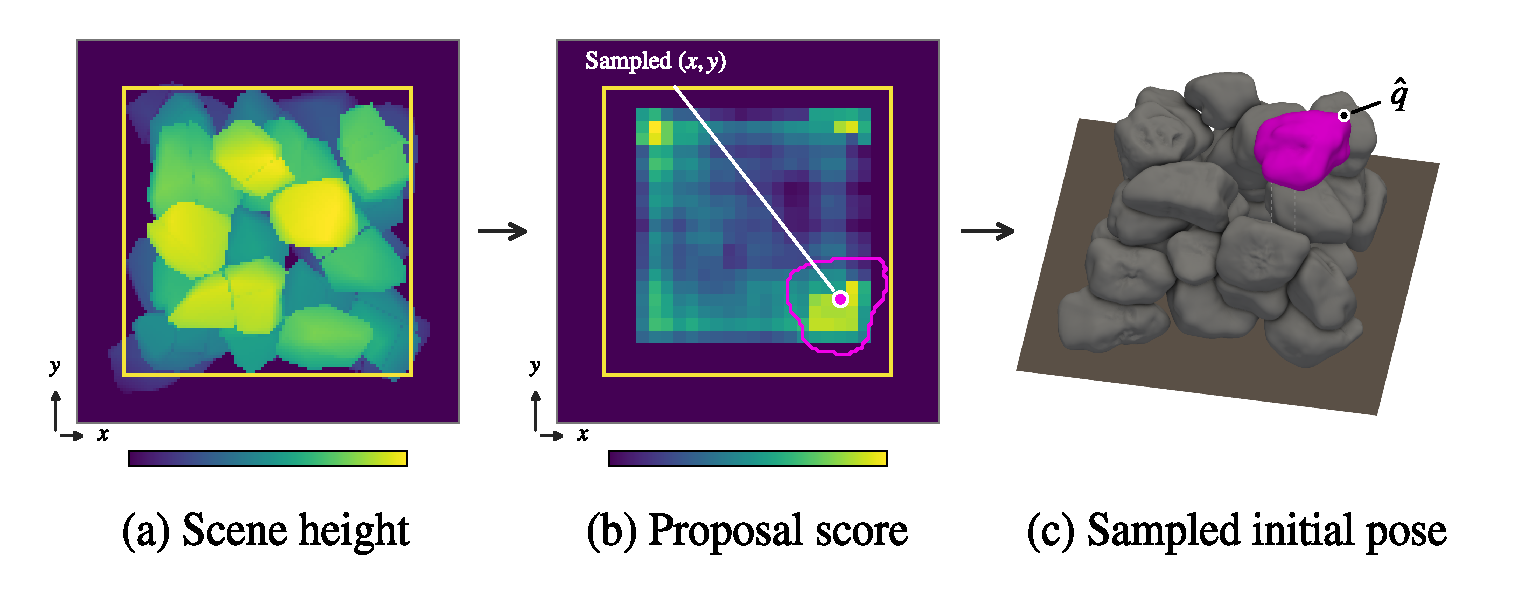
\includegraphics[width=\columnwidth]{figures/initial_pose_sampling.eps}
  \caption{Initial pose sampling for a fixed object and orientation: (a) scene height, (b) proposal score and sampled planar location, and (c) initial pose $\hat q$ above the scene. Magenta links the sampled location and candidate object.}
  \label{fig:score_map}
\end{figure}


\subsection{Reward Design}\label{sec:reward}
For the new object $i=i_{k+1}$ at its settled successor pose $q_i'$ (Sec.~\ref{sec:simulation}), define
\begin{equation*}
 \rho_\target=\frac{\vol\bigl(\object_i(q_i')\cap\target\bigr)}{\vol(\target)},
 \quad
 \rho_\object=\frac{\vol\bigl(\object_i(q_i')\cap\target\bigr)}{\vol(\object_i)}.
\end{equation*}
These voxel-estimated ratios reward target volume filling and containment. For feasible transitions,
\begin{equation*}
\begin{split}
 r(\state,\action)={}&w_\target\rho_\target+w_\object[\rho_\object-\tfrac12]_+
 -w_E e(\action)\\
 &+w_H\bigl(\phi_H(\state)-\phi_H(\state')\bigr)
 -w_D D,
\end{split}
\end{equation*}
where $\phi_H(s)=\operatorname{Var}_\Omega(H_s)$ is the area-weighted variance of scene height over the target footprint $\Omega$, with empty cells assigned zero height.
Loss of occupied volume within the target due to motion of previously placed objects is not subtracted. Failed transitions receive $r=-1$.

For pose-optimization residual forces $\mathbf f_l$ and torques $\boldsymbol\tau_l$ across all placed objects,
\begin{equation*}
 e(\action)=\max_l\left(
 \frac{\|\mathbf f_l\|}{m_lg}
 +\frac{\|\boldsymbol\tau_l\|}{m_lg\vol(\object_l)^{1/3}}\right).
\end{equation*}
Candidates with $e(\action)\geq\epsilon_\mathrm{eq}$ are rejected before simulation.
Disturbance sensitivity measures motion from settled poses $q_l'$ during force trials:
\begin{equation*}
 D=\min\!\left\{D_{\max},\max_{j,l,t}d_{\SE(3)}\bigl(q_l^{(j)}(t),q_l'\bigr)\right\}.
\end{equation*}
Here $q_l^{(j)}(t)$ is the pose of object $l$ at time $t$ in trial $j$, including recovery; $d_{\SE(3)}$ sums translation distance and angular distance scaled by $\lambda_\theta>0$.
